% -----------------------------*- LaTeX -*------------------------------
\documentclass[11pt]{report}
\usepackage{ds603_scribe}
\usepackage{xcolor}
\usepackage{amsmath, amssymb, amsthm}
\usepackage{algorithm}
\usepackage{algorithmic}
\usepackage{graphicx}
\usepackage{enumitem}

\newcommand{\ab}[1]{\textcolor{purple}{[#1 - AB]}}
\newcommand{\abedit}[1]{\textcolor{purple}{#1}}

\begin{document}

\scribe{Adwai Krishna}		% required
\lecturenumber{12}			% required
\lecturedate{03/10/2025}	% required

\maketitle

% ----------------------------------------------------------------------

\section{Adversarial Attacks: Min-Norm and Query-Based}

\subsection*{Introduction}
Adversarial attacks are deliberate perturbations to input data at test time that aim to fool machine learning into making incorrect predictions. These perturbations are typically small and often imperceptible to humans, yet can drastically alter model outputs.

In this lecture, we will cover adversarial attacks of two categories:
\begin{enumerate}
    \item \textbf{Min-Norm Based Attacks:} Optimization-based methods minimizing perturbation norm while achieving misclassification.
    \item \textbf{Query-Based Attacks:} With access only to classifier outputs, how to construct effective adversarial examples.
\end{enumerate}

\section{Min-Norm Based Adversarial Attacks}

\subsection*{Optimization Problem Formulation}
Given a classifier $h_\theta: X=\mathbb{R}^d \to \{1, \dots, K\}$ and input $x$, the goal is to find the smallest perturbation $\delta$ such that
\[
    h_\theta(x + \delta) \neq h_\theta(x),
\]
or equivalently,
\[
\min_{\delta \in X} \|\delta\|_2
\quad\text{s.t.}\quad
\begin{aligned}
  & h_\theta(x+\delta) \neq h_\theta(x), \\[1.2ex] % <-- extra vertical space
  & x+\delta \in X
\end{aligned}
\]
\\
Note: The issue here is that it is difficult to optimize over this constraint set.

\subsection*{Conversion to Unconstrained Optimization}
Transforming the constrained problem into an unconstrained form:
\[
    \min_{\delta \in X} \|\delta\|_2 + \lambda \cdot g(x + \delta) \quad \text{s.t.} \quad x+\delta \in X
\]
What should $g(.)$ be such that it captures the constraint best?
\[
    \text{Choose} \quad g(.) \quad \text{s.t.} \quad g(.) \leq 0 \quad \iff \quad h_\theta(x+\delta) \neq h_\theta(x)
\]
Other possibilities of $g(.)$ are discussed later.

\subsection*{Differentiable Constraint Approximation}
We define the following surrogate function
\[
    g(x+\delta) = \max[f_\theta(x+\delta)_y - \max_{i \neq y} f_\theta(x+\delta)_i, -\kappa],
\]
where $f_\theta(x)$ is the classifier score (logits) and $\kappa$ controls the confidence margin.

\subsection*{Box Constraint Handling}
Note: In practice, $x+\delta$ can only lie in some pre-specified box constraint. For example, images lie in  $[0,1]^d$, which leads to box-constrained optimization. \\
To ensure box constraints, we use a \textbf{change of variable} as follows:
\[
    \delta_i = \frac{1}{2}(\tanh(w_i) + 1) - x_i,
\]
\[
    \implies x_i + \delta_i = \frac{1}{2}(\tanh(w_i) + 1)
\]
Note: $tanh(.) \in [-1,1]$

\subsection*{Carlini \& Wagner - $L_2$ Norm Attack}

We perform optimization over $w$

\[
    \min_w \left\|\frac{1}{2}(\tanh(w) + 1) - x\right\|_2 + \lambda \cdot \max\left[f_\theta\left(\frac{1}{2}(\tanh(w) + 1)\right)_y - \max_{i \neq y} f_\theta\left(\frac{1}{2}(\tanh(w) + 1)\right)_i, -\kappa\right]
\]

\subsection*{Carlini \& Wagner - $L_\infty$ Norm Attack}
Comparing with the $L_2$ norm case, in $L_\infty$,
\[
    \text{the term } \left\|\frac{1}{2}(\tanh(w) + 1) - x\right\|_2 \text{ becomes } \sum_{i=1}^d [(\delta_i-\tau_t)^+] \quad \text{(slack for each $\delta_i$)},
\]
where $\tau_t$ is an iteration-dependent hyperparameter. \\
Now the question arises: Should we increase or decrease $\tau_t$ in each iteration? $->$ We should decrease it.

\subsubsection*{Other Options for $g(.)$}
Option 1:
\[
    g(.) = l_{surr}(x+\delta, y)
\]
Option 2:
\[
    g(.) = \max[\text{softmax}(f_\theta(x+\delta)_y) - \max_{i \neq y} \text{softmax}(f_\theta(x+\delta)_i), -\kappa],
\]

\section{Query-Based Adversarial Attacks}

\subsubsection*{Revisiting Notations}

\[
\begin{aligned}
    & h_\theta : X \xrightarrow{} [i]_{i=1}^c, \\
    & s_\theta : X \xrightarrow{} [0,1]^{\lvert c \rvert}, \\
    & f_\theta: X \xrightarrow{} \mathbb{R}^{\lvert c \rvert}, \\
    & h_\theta = \arg\max_i (s_\theta)_i, \\
    & s_\theta = \text{softmax}(f_\theta) \implies (s_\theta)_i = \frac{e^{(f_\theta)_i}}{\sum_{i=1}^c e^{(f_\theta)_i}}
\end{aligned}
\]

\subsubsection*{Threat Model}
Two main types of query-based black-box attacks:
\begin{itemize}
    \item Score-based: Access to $s_\theta$ is available.
    \item Decision-based: Only access to $h_\theta$ is available.
\end{itemize}

\subsection{Score-Based Attacks}
Assume that the loss function of interest depends on either $s_\theta$ or $f_\theta$, for example, cross-entropy or hinge loss.
\[
\begin{aligned}
    & l_{CE}((\vec{x}, y), s_\theta) = -\log(s_\theta)_y \quad \text{(assuming hard labels)} \\
    & l_{Hinge}((\vec{x}, y), f_\theta) = \max (0, 1-y \cdot f_\theta(\vec{x}))
\end{aligned}
\]
To construct adversarial examples using CE loss, we need
\[
    \nabla_{\vec{x}} l_{CE} = \nabla_{\vec{x}} (-\log(s_\theta)_y) = -\frac{1}{(s_\theta)_y} \cdot (\nabla_{\vec{x}} (s_\theta)_y)
\]
\\
For simplicity, let $(s_\theta)_y = s$, so we need to estimate $\nabla_{\vec{x}} s$.
\\
Now, for any function $s$, its \textbf{directional derivative} along a vector $\vec{u}$ is
\[
    \nabla_{\vec{u}} s(\vec{x}) = \lim_{\alpha \to 0} \frac{s(\vec{x}+\alpha\vec{u}) - s(\vec{x})}{\alpha\|\vec{u}\|} = \lim_{\alpha \to 0} \frac{s(\vec{x}+\alpha\vec{u}) - s(\vec{x})}{\alpha} \text{ if } \|\vec{u}\| = 1
\]
\\
Furthermore, if $s$ is differentiable, then
\[
     \nabla_{\vec{u}} s(\vec{x}) = \nabla s(\vec{x})^T \cdot \vec{u}
\]

\subsubsection*{Zeroth Order Optimization}

The choice of direction will determine the algorithm that can be used.\\
If $\vec{u} = \vec{e_i}$, then the directional derivative is just $\frac{ds}{d\vec{x_i}}$
\[
    \nabla_{\vec{e_i}} s(\vec{x}) = \frac{ds}{d\vec{x_i}} = \lim_{\alpha \to 0} \frac{s(\vec{x}+\alpha\vec{e_i}) - s(\vec{x})}{\alpha} \approx \frac{s(\vec{x}+\alpha\vec{e_i}) - s(\vec{x})}{\alpha} = \hat{\nabla}_{\vec{x}}s(\vec{x})
\]
\\
Now we have 2 options:
\begin{itemize}
    \item \textbf{Option 1}: Do this $d$ times and use stochastic gradient descent
    \begin{itemize}
        \item Recall that for a convex, Lipschitz function, the rate is $\frac{RL}{\sqrt{t}}$, where $R$ is the radius of the ball and $L$ is the Lipschitz constant.
        \item $\frac{RL}{\sqrt{t}} \leq \epsilon \implies t \geq \frac{R^2L^2}{\epsilon^2}$
        \item So, number of queries $\xrightarrow{} O(d\frac{R^2L^2}{\epsilon^2})$
    \end{itemize}
    \item \textbf{Option 2}: Use Stochastic/Random Coordinate Descent
\end{itemize}

\subsubsection*{Stochastic/Random Coordinate Descent (S/RCD)}
Step: $\vec{x}_{t+1} = \vec{x}_t - \eta \nabla_{\vec{e_i}} s(\vec{x}) \: \vec{e_i}$, \\ where $i$ is drawn uniformly at random from $[d]$ 
\\
\\
\textbf{Theorem}: If $s$ is convex and L-Lipschitz, then S/RCD satisfies 
\[
    \mathbb{E} \: s\Big(\frac{1}{T}\sum_{t=1}^T \vec{x}_t\Big) - \inf_{\vec{x} \in X} s(\vec{x}) \leq \frac{RL}{\sqrt{t}}\sqrt{d}
\]
\\
So in S/RCD
\[
    \frac{RL}{\sqrt{t}}\sqrt{d} \leq \epsilon \implies t \geq \frac{R^2L^2}{\epsilon^2} d
\]
\\
So, number of queries $\xrightarrow{} O(d\frac{R^2L^2}{\epsilon^2})$, ending up with the same penalty as option 1.

\noindent
\textbf{Note:} To get the same accuracy, RCD requires $d$ times more iterations. So, if $s$ is convex and $L$-Lipschitz, both options will be equally good (GD and RCD).
\\
\\
We can speed this up by batching and updating $B$ randomly chosen coordinates in each step, i.e. $\vec{u} = \frac{1}{\sqrt{B}}e_I$ where $\lvert I \rvert = B$. 
This implies we are estimating
\[
    \nabla_{\vec{u}} \: s(\vec{x}) = \nabla s(\vec{x})^T \vec{u}, \quad \text{with} \quad \vec{u} = \frac{1}{\sqrt{B}} \sum_{i \in I} \frac{ds(\vec{x})}{d\vec{x}_i},
\]
which is just the average partial derivative along the chosen directions.
\subsubsection*{Gaussian Random Vectors}
$\vec{u}$ can be chosen based on a draw from a $d$-dimensional Gaussian distribution, $\vec{u} \sim \mathcal{N}(0, I_d)$, giving the approximation
\[
    \widehat{\nabla}_{\vec{x}} \: s(\vec{x}) = \frac{s(\vec{x} + \delta \vec{u}) - s(\vec{x})}{\delta} .
\]
\subsubsection*{Simultaneous Perturbation Stochastic Approximation}
A general iterative procedure for minimization is as follows:
\begin{equation}
    \vec{x}_{t+1} = \vec{x}_t - w_t \Big[ \frac{s(\vec{x_t} + \delta_t \vec{u_t}) - s(\vec{x_t})}{\delta_t} \Big] \vec{u_t},
\end{equation}
Denote $\Big[\frac{s(\vec{x_t} + \delta_t \vec{u_t}) - s(\vec{x_t})}{\delta_t}\Big] \vec{u_t} = \widehat{\nabla}_{\delta_t} \: s(\vec{x_t})$.
\\
\\
Suppose $s$ is convex and we want to solve
\[
    \inf_{\vec{x} \in X} s(\vec{x}) \quad (:= s^*).
\]
\\
\textbf{Note:} In the untargeted problem, we actually do ascent, but let us assume here that we are in the targeted version, where we would solve $\inf_{\vec{x'} \in X} \tilde{s}(\vec{x'})_T$, where $T$ is the target class.
\subsubsection*{Gradient-Free Optimization Convergence (Nesterov and Spokoiny, 2015)}
\textbf{Theorem:} Let $\{\vec{x_t}\}_{t \geq 0}$ be the sequence of generated iterates following procedure (1) and let $\beta_T = \sum_{t=0}^{T} w_t$. Then for any $T \ge 0$, we have
\[
    \frac{1}{\beta_T} \sum_{t=0}^{T} w_t \phi_t - s^* \le \delta L \sqrt{d} + \frac{1}{\beta_t}\Big[\frac{1}{2}\|\vec{x}_0 - \vec{x*}\|^2 + \frac{(d+4)^2}{2} L^2 \sum_{t=0}^{T} h_t^2 \Big] ,
\]
where $\phi_t = \mathbb{E}_{[\vec{u_t}]_{t=0}^{T-1}} \Big[ s(\vec{x_t}) \Big]$.
\\
\\
\textbf{Note:} To get error $\epsilon_s$, choose $\delta \le \frac{\epsilon}{2L\sqrt{d}}$ and $T = \frac{4 (d+4)^2}{\epsilon^2}L^2R^2$.


\subsection{An Example}

\begin{figure}[h!]
    \centering

    % --- First image (clean) ---
    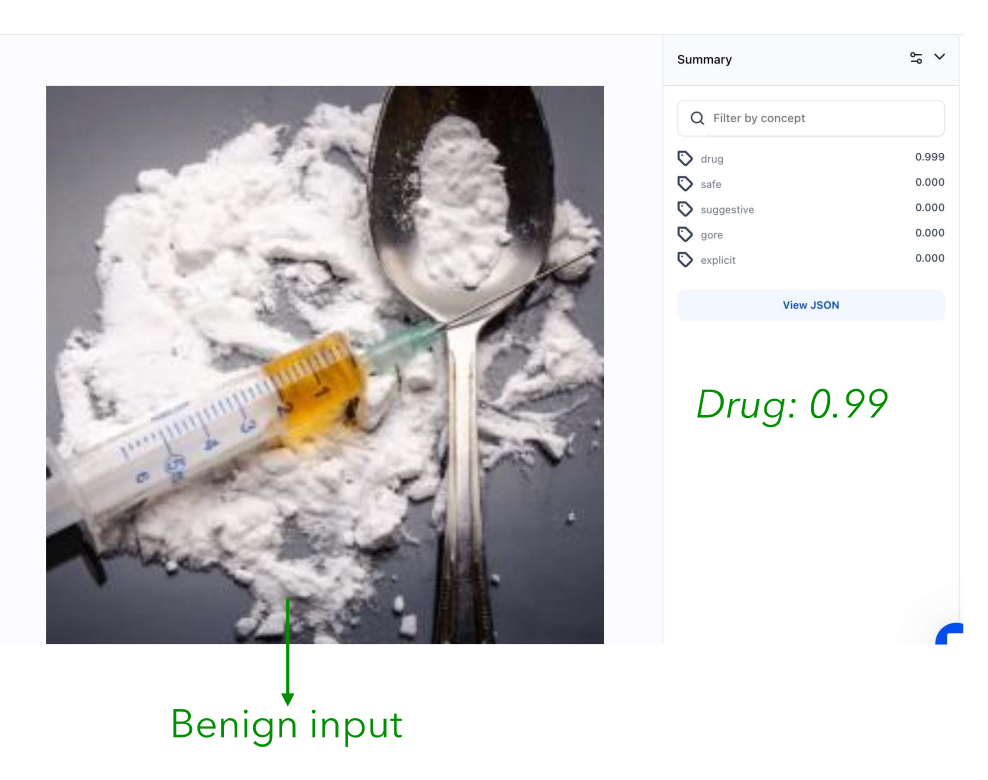
\includegraphics[width=0.7\linewidth]{imgs/img1.png}
    \vspace{0.5em}
    \caption*{(a) Original (clean) input image}

    % --- Second image (adversarial) ---
    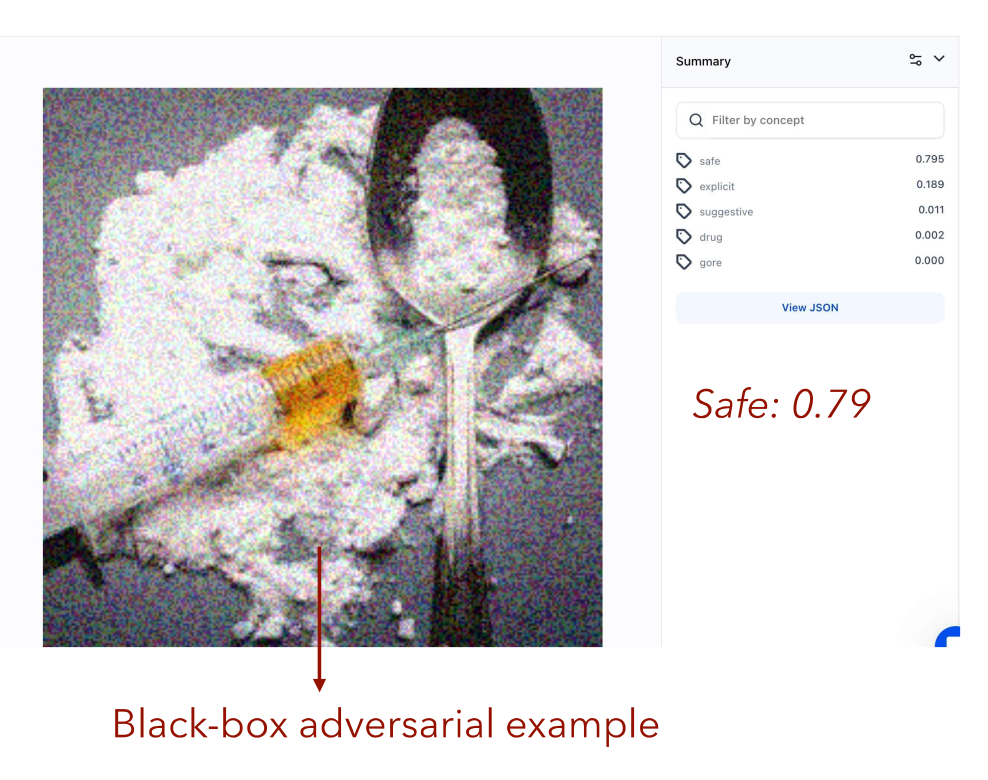
\includegraphics[width=0.7\linewidth]{imgs/img2.png}
    \vspace{0.5em}
    \caption*{(b) Adversarially perturbed image}

    \caption{Comparison of clean and adversarial image. 
    The adversarial image remains visually similar but leads to misclassification.}
    \label{fig:adv_comparison}
\end{figure}



\nocite{nesterov2015random}
\nocite{carlini2017towards}


\bibliographystyle{plain}
\bibliography{refs}

\end{document}
